%----------------------------------------------------------------------------------------
%	PACKAGES AND OTHER DOCUMENT CONFIGURATIONS
%----------------------------------------------------------------------------------------

\documentclass[12pt]{article}

%%%%%%%%%%%%%%%%%%%%%%%%%%%%%%%%%%%%%%%%%
% Lachaise Assignment
% Structure Specification File
% Version 1.0 (26/6/2018)
%
% This template originates from:
% http://www.LaTeXTemplates.com
%
% Authors:
% Marion Lachaise & François Févotte
% Vel (vel@LaTeXTemplates.com)
%
% License:
% CC BY-NC-SA 3.0 (http://creativecommons.org/licenses/by-nc-sa/3.0/)
% 
%%%%%%%%%%%%%%%%%%%%%%%%%%%%%%%%%%%%%%%%%

%----------------------------------------------------------------------------------------
%	PACKAGES AND OTHER DOCUMENT CONFIGURATIONS
%----------------------------------------------------------------------------------------

\usepackage{amsmath,amsfonts,stmaryrd,amssymb} % Math packages

\usepackage{enumerate} % Custom item numbers for enumerations

\usepackage[ruled]{algorithm2e} % Algorithms

\usepackage[framemethod=tikz]{mdframed} % Allows defining custom boxed/framed environments

\usepackage{listings} % File listings, with syntax highlighting
\lstset{
	basicstyle=\ttfamily, % Typeset listings in monospace font
}

%----------------------------------------------------------------------------------------
%	DOCUMENT MARGINS
%----------------------------------------------------------------------------------------

\usepackage{geometry} % Required for adjusting page dimensions and margins

\geometry{
	paper=a4paper, % Paper size, change to letterpaper for US letter size
	top=2.5cm, % Top margin
	bottom=3cm, % Bottom margin
	left=2.5cm, % Left margin
	right=2.5cm, % Right margin
	headheight=14pt, % Header height
	footskip=1.5cm, % Space from the bottom margin to the baseline of the footer
	headsep=1.2cm, % Space from the top margin to the baseline of the header
	%showframe, % Uncomment to show how the type block is set on the page
}


%----------------------------------------------------------------------------------------
%	COMMAND LINE ENVIRONMENT
%----------------------------------------------------------------------------------------

% Usage:
% \begin{commandline}
%	\begin{verbatim}
%		$ ls
%		
%		Applications	Desktop	...
%	\end{verbatim}
% \end{commandline}

\mdfdefinestyle{commandline}{
	leftmargin=10pt,
	rightmargin=10pt,
	innerleftmargin=15pt,
	middlelinecolor=black!50!white,
	middlelinewidth=2pt,
	frametitlerule=false,
	backgroundcolor=black!5!white,
	frametitle={Command Line},
	frametitlefont={\normalfont\sffamily\color{white}\hspace{-1em}},
	frametitlebackgroundcolor=black!50!white,
	nobreak,
}

% Define a custom environment for command-line snapshots
\newenvironment{commandline}{
	\medskip
	\begin{mdframed}[style=commandline]
}{
	\end{mdframed}
	\medskip
}

%----------------------------------------------------------------------------------------
%	FILE CONTENTS ENVIRONMENT
%----------------------------------------------------------------------------------------

% Usage:
% \begin{file}[optional filename, defaults to "File"]
%	File contents, for example, with a listings environment
% \end{file}

\mdfdefinestyle{file}{
	innertopmargin=1.6\baselineskip,
	innerbottommargin=0.8\baselineskip,
	topline=false, bottomline=false,
	leftline=false, rightline=false,
	leftmargin=2cm,
	rightmargin=2cm,
	singleextra={%
		\draw[fill=black!10!white](P)++(0,-1.2em)rectangle(P-|O);
		\node[anchor=north west]
		at(P-|O){\ttfamily\mdfilename};
		%
		\def\l{3em}
		\draw(O-|P)++(-\l,0)--++(\l,\l)--(P)--(P-|O)--(O)--cycle;
		\draw(O-|P)++(-\l,0)--++(0,\l)--++(\l,0);
	},
	nobreak,
}

% Define a custom environment for file contents
\newenvironment{file}[1][File]{ % Set the default filename to "File"
	\medskip
	\newcommand{\mdfilename}{#1}
	\begin{mdframed}[style=file]
}{
	\end{mdframed}
	\medskip
}

%----------------------------------------------------------------------------------------
%	NUMBERED QUESTIONS ENVIRONMENT
%----------------------------------------------------------------------------------------

% Usage:
% \begin{question}[optional title]
%	Question contents
% \end{question}

\mdfdefinestyle{question}{
	innertopmargin=1.2\baselineskip,
	innerbottommargin=0.8\baselineskip,
	roundcorner=5pt,
	nobreak,
	singleextra={%
		\draw(P-|O)node[xshift=1em,anchor=west,fill=white,draw,rounded corners=5pt]{%
		Question \theQuestion\questionTitle};
	},
}

\newcounter{Question} % Stores the current question number that gets iterated with each new question

% Define a custom environment for numbered questions
\newenvironment{question}[1][\unskip]{
	\bigskip
	\stepcounter{Question}
	\newcommand{\questionTitle}{~#1}
	\begin{mdframed}[style=question]
}{
	\end{mdframed}
	\medskip
}

%----------------------------------------------------------------------------------------
%	WARNING TEXT ENVIRONMENT
%----------------------------------------------------------------------------------------

% Usage:
% \begin{warn}[optional title, defaults to "Warning:"]
%	Contents
% \end{warn}

\mdfdefinestyle{warning}{
	topline=false, bottomline=false,
	leftline=false, rightline=false,
	nobreak,
	singleextra={%
		\draw(P-|O)++(-0.5em,0)node(tmp1){};
		\draw(P-|O)++(0.5em,0)node(tmp2){};
		\fill[black,rotate around={45:(P-|O)}](tmp1)rectangle(tmp2);
		\node at(P-|O){\color{white}\scriptsize\bf !};
		\draw[very thick](P-|O)++(0,-1em)--(O);%--(O-|P);
	}
}

% Define a custom environment for warning text
\newenvironment{warn}[1][Warning:]{ % Set the default warning to "Warning:"
	\medskip
	\begin{mdframed}[style=warning]
		\noindent{\textbf{#1}}
}{
	\end{mdframed}
}

%----------------------------------------------------------------------------------------
%	INFORMATION ENVIRONMENT
%----------------------------------------------------------------------------------------

% Usage:
% \begin{info}[optional title, defaults to "Info:"]
% 	contents
% 	\end{info}

\mdfdefinestyle{info}{%
	topline=false, bottomline=false,
	leftline=false, rightline=false,
	nobreak,
	singleextra={%
		\fill[black](P-|O)circle[radius=0.4em];
		\node at(P-|O){\color{white}\scriptsize\bf i};
		\draw[very thick](P-|O)++(0,-0.8em)--(O);%--(O-|P);
	}
}

% Define a custom environment for information
\newenvironment{info}[1][Info:]{ % Set the default title to "Info:"
	\medskip
	\begin{mdframed}[style=info]
		\noindent{\textbf{#1}}
}{
	\end{mdframed}
}
 % Include the file specifying the document structure and custom commands

%----------------------------------------------------------------------------------------
%	ASSIGNMENT INFORMATION
%----------------------------------------------------------------------------------------

\title{\textbf{An Investigation into Predicting Reading Preferences}} % Title of the assignment

\author{Maths AI HL Internal Assessment} % Author name and email address
%----------------------------------------------------------------------------------------

\begin{document}

\doublespacing

\maketitle % Print the title
\thispagestyle{empty}
\pagebreak
\tableofcontents
\thispagestyle{empty}

\clearpage
\pagenumbering{arabic}

\pagebreak
\section{Introduction} % Unnumbered section

Reading is one of those particular hobbies that has stuck with me over the years, despite the
changes I have undergone as a person. My fervent passion for this hobby is demonstrated
through my purchase and constant use of a Kindle, the second-hand bookshop loyalty cards
stashed in my pencil case, and my notebook dedicated to logging words, quotes and the
books I have read. Naturally, my taste and reasons for reading have changed over time, and
I have attempted to find ways in which I could express this development concretely.

Although I have an intuitive sense of whether I will enjoy a book, it is challenging to reify
something as abstract and complex as book preference -- there are many contributing factors
and they all have varying influences. Although there exists a variety of recommendation
engines online, these often rely on majority preference, and in my personal opinion, are not
nuanced or representative enough of an individual's personal tastes.

For this reason, the focus of this IA will be to build a simplified, however, more personalised
book preference model, where a mixture of both primary and secondary data will be collated
to create a model that can predict whether I will enjoy a book based on my past read books.

The more technical objective of this IA is to create a graphical representation where my past
read books are represented as points; the Euclidian distances between them represent
similarity (in terms of the likelihood of enjoying a book), which are then used to form
“likelihood of preference” groups.

\subsection{Aim}
The objectives detailed above can be simplified into the following aim:

\textit{Attempt to graphically represent my books based on factors that personally determine a book’s “quality” and categorize these into “likely to be enjoyed” and “unlikely to be enjoyed” groups.}

\section{Dataset}
Overall, twelve factors were determined to be the characteristics I personally found were
important in determining whether I would enjoy a book. This information (primary and
secondary) was collated and presented here below:


\begin{table}[!htbp]
    \centering
    \begin{tabular}{|p{7cm}|p{7cm}|}
        \hline
        \textbf{Primary Data} & \textbf{Secondary Data}\\
        \hline
        1. Book Title & 4. Year Published \\
        2. Book Author & 5. Average Rating \\
        3. Personal Rating & 6. Number of Votes \\
        & 7. Number of Pages \\
        & 8. Dark \% \\
		& 9. Challenging \% \\
		& 10. Reflective \% \\
		& 11. Sad \% \\
		& 12. Tense \% \\
        \hline
    \end{tabular}
    \caption{Tabled Primary \& Secondary Data}
\end{table}

The primary data comes from a personal book log I have kept for the past 1.5 years. It
includes the \textbf{book titles}, their respective \textbf{authors}, and my \textbf{personal rating} of each book.

The secondary data was collected from Goodreads and TheStoryGraph -- two popular
websites used to track books read and obtain recommendations. From Goodreads, the \textbf{year
published, number of pages, average rating} as well as the \textbf{number of users} that
provided that rating. As for TheStoryGraph, the website's reading analysis function was
utilized to indicate my top read and preferred moods/themes in books. The top five were
selected and used as part of the model: \textbf{Dark, challenging, reflective, tense}, and \textbf{sad}. For
each book on the site, users can submit a review where they rate certain moods' presence in
a book. For instance, a book dealing with themes of remorse and grief would have high
mood percentages in “sad”, “dark”, and “tense”. For each book in the log, the mood
percentages for the 5 mentioned moods were obtained.

Overall \textbf{43 book entries} are used to create the model. A sample snippet of the tabled data is
presented here below:

\begin{figure}[H]
	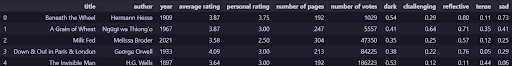
\includegraphics[width=\textwidth]{1}
	\centering
	\caption{Raw Data Snippet}
\end{figure}

\section{Methodology}

\underline{Math Employed} - Linear combinations, covariance matrices, eigenvectors, eigenvalues, Voronoi diagrams, PCA, KMeans clustering.

\subsection{Technology}
Due to the dataset’s relatively large size, it would be impractical and inefficient to carry out on every
individual entry the calculations needed to address this IA’s aims. 
Hence, \textit{Python 3.12} is used alongside \textit{Jupyter Notebooks} to facilitate this process. 
The following 3rd party external libraries were also used as part of generating the 
graphics and performing specific calculations: \textit{Sklearn, Numpy, Matplolib} and \textit{Pandas}. 
Throughout this IA, comments explaining the code snippets will be denoted by the \# preceding the explanations.

\subsection{Procedure Overview}
\begin{question}[\bf{Modelling Steps}]
    \begin{enumerate}
    \itemsep -1em 
        \item Load, organise data into tables and standardise.
        \item Perform PCA (Principal Component Analysis) with $n = 2$.
        \item Scatter plot the $2$ principal components.
        \item Determine outlying points.
        \item Scatter plot the $2$ principal components again, without the outliers.
        \item Visually analyze book scatterplot to estimate book distribution and groups.
        \item Use KMeans clustering to generate cluster centre points.
        \item Plot cluster centre points.
        \item Construct a Voronoi diagram to form category cells.
    \end{enumerate}
\end{question}

\section{Steps}
\subsection{Step 1: Load, organise data into tables and standardise}
All the primary and secondary data were manually collated and stored in a CSV file. This was then loaded into the Python file to yield the table shown in the \textit{Dataset} section.

As can be seen from the table output, there is a mixture of quantitative and qualitative data. Furthermore, the numerical data varies in units and magnitudes, which will affect PCA later on, as it works based on the data’s variability, so leaving the data unprocessed will yield problems later on. This issue is addressed by centring and standardising the data. This involves making the mean of the data 0, and the standard deviation 1.

Firstly, all the numerical data from the dataset is extracted and stored separately (10 factors overall). For each factor in the dataset, all the values were taken and their mean and standard deviation were calculated. The mean was then subtracted from each value and was then divided by the standard deviation. The programmed process and output table are presented here below:

\begin{figure}[H]
	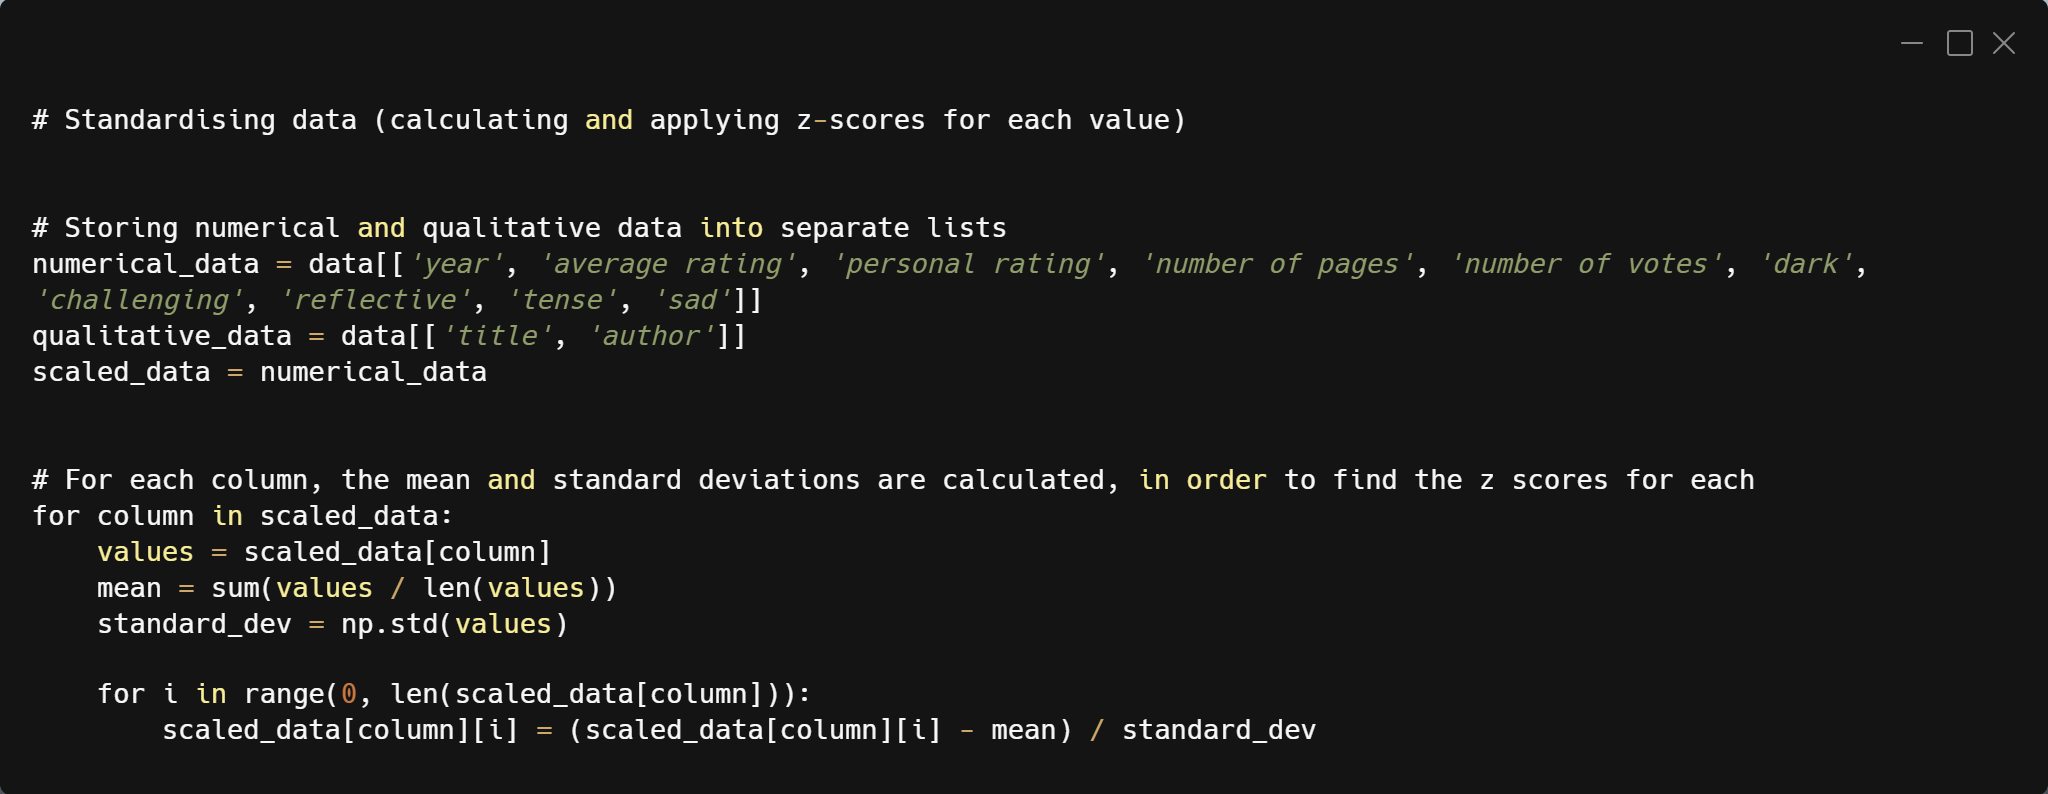
\includegraphics[width=\textwidth]{code1}
	\centering
	\caption{Code for standardisation of data}
\end{figure}

\begin{figure}[H]
	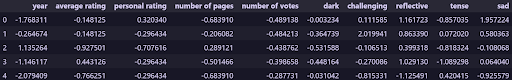
\includegraphics[width=\textwidth]{2}
	\centering
	\caption{Snippet of resulting scaled data table}
\end{figure}

\subsection{Step 2: Perform PCA with n = 2}
PCA (Principal Component Analysis) is a dimensionality reduction technique. The first aim of this IA involves graphically presenting the books, however, currently, each book is associated with 10 different variables. It can be said that the dataset has 10 dimensions. Since humans are only able to visually process a maximum of 3 dimensions, graphing 10 different variables would prove to be difficult to understand. PCA addresses this problem by \textbf{reducing the number of variables while preserving as much data as possible}.
\parencite{1} The method in which this process is carried out is as follows:

\begin{enumerate}
    \item Identify the number of dimensions to reduce the data to ($2$ or $3$ for visualisation). For the purposes of this IA, $2$ dimensions will be chosen.
    \item This technique involves examining how variables relate to each other which often includes additional redundant information which can be taken out to reduce the dataset’s dimensionality. Firstly, to identify correlations between the variables, a covariance matrix is calculated. This is a square matrix, where each entry is the covariance of two variables. Overall, this matrix will contain all the covariances of all the possible variable combinations from the dataset.
    \item To obtain the $2$ dimensions that are then plotted, the eigenvectors and eigenvalues are computed from that previously computed covariance matrix. This yields the \textbf{principal components} which are then graphed. These in themselves do not hold real meaning as they do not represent a particular unit or magnitude. Rather, these are \textbf{linear combinations} of the original data.
\end{enumerate}

The programmed process and principal component coordinates obtained for each book are presented below:

\begin{figure}[H]
	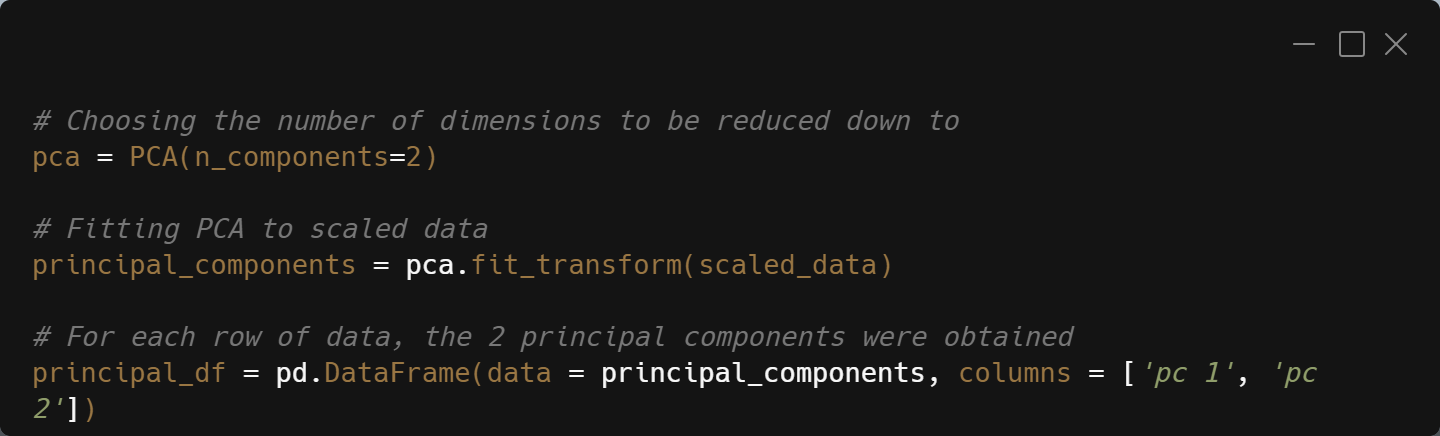
\includegraphics[width=\textwidth]{code2}
	\centering
	\caption{Code for PCA}
\end{figure}
\vspace{-1em}
\begin{figure}[H]
	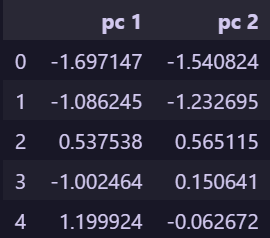
\includegraphics[scale=0.4]{3}
	\centering
	\caption{Snippet of resulting principal components table}
\end{figure}

\subsection{Step 3: Scatter plot the 2 principal components}
The obtained principal component coordinates for each book were then plotted. The two plots, one with and one without the labelled book titles are presented below:

\begin{figure}[H]
	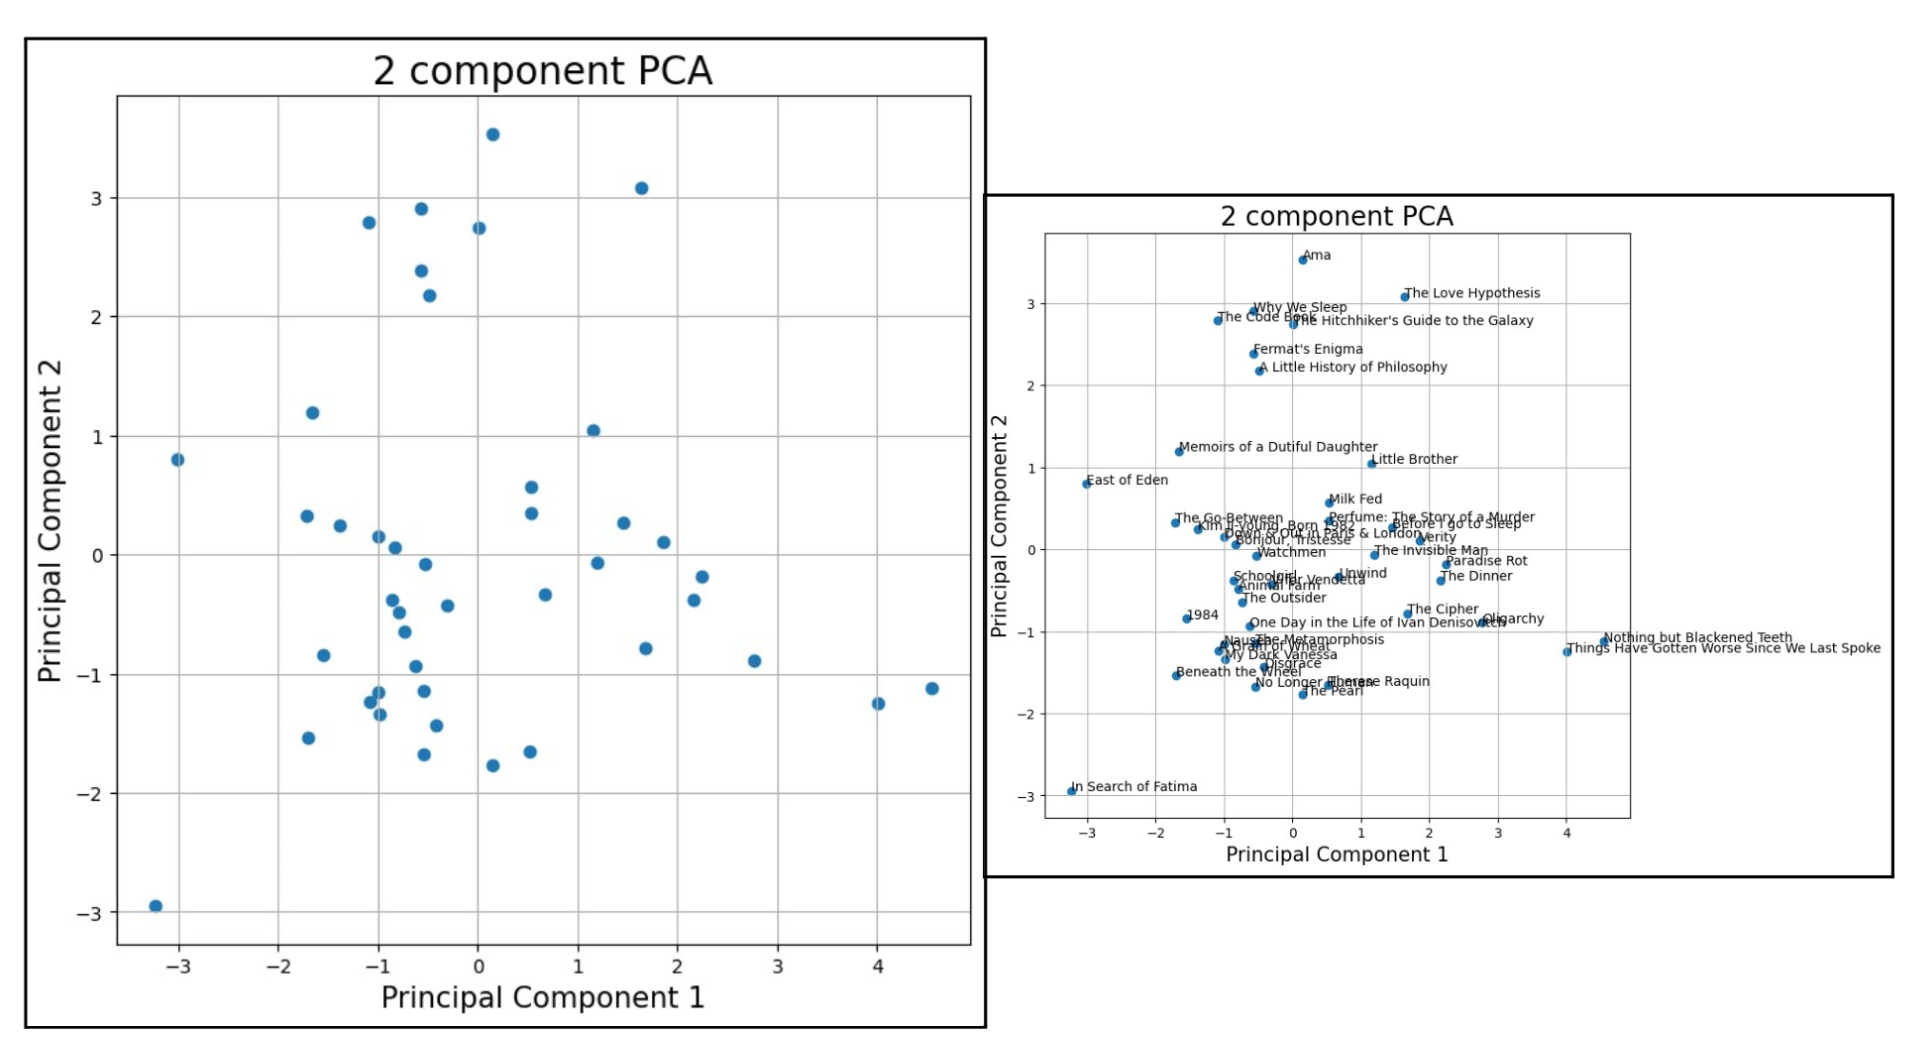
\includegraphics[scale=0.4]{4}
	\centering
	\caption{PCA unlabelled \& labelled plots}
\end{figure}

\subsection{Step 4: Determine outlying points}
Visually, from the plot above, it can be seen that certain points (such as “In Search of Fatima”) are generally much further away from the rest of the points. Thus, an outlier test was performed to confirm this. Since the year published, the number of pages, number of votes, average rating, and my personal rating are constants, only the outliers for the mood percentages are calculated. The interquartile range was calculated for the $5$ moods and the outliers identified by the books that deviated from that range. The programmed process, as well as the identified outliers, are presented below:
\begin{figure}[H]
	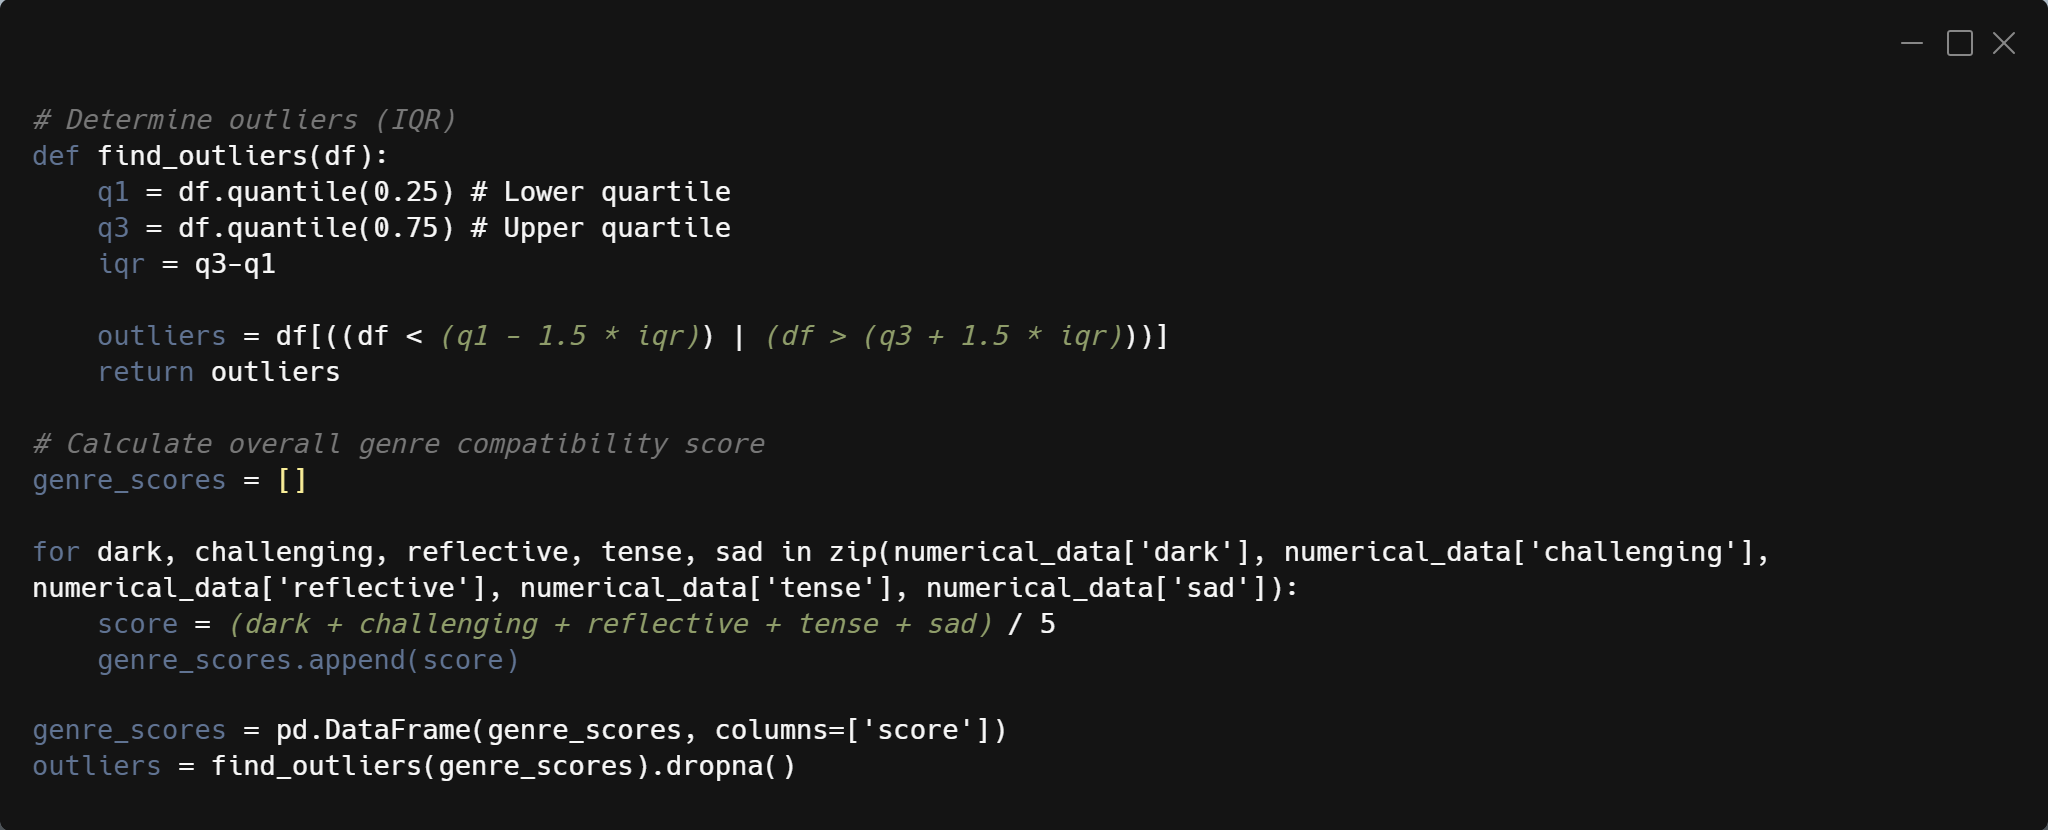
\includegraphics[width=\textwidth]{code3}
	\centering
	\caption{Code for determining outliers}
\end{figure}
\vspace{-1em}
\begin{figure}[H]
	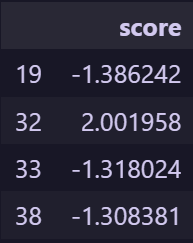
\includegraphics[scale=0.4]{5}
	\centering
	\caption{Resulting identified outliers table}
\end{figure}

\subsection{Step 5: Scatter plot the 2 PCs without outliers}
The $4$ books identified to be outliers are then omitted from the dataset and replotted. Below is presented the programmed process, the “before” scatterplot with outliers highlighted, and the “after” graph with outliers omitted:

\begin{figure}[H]
	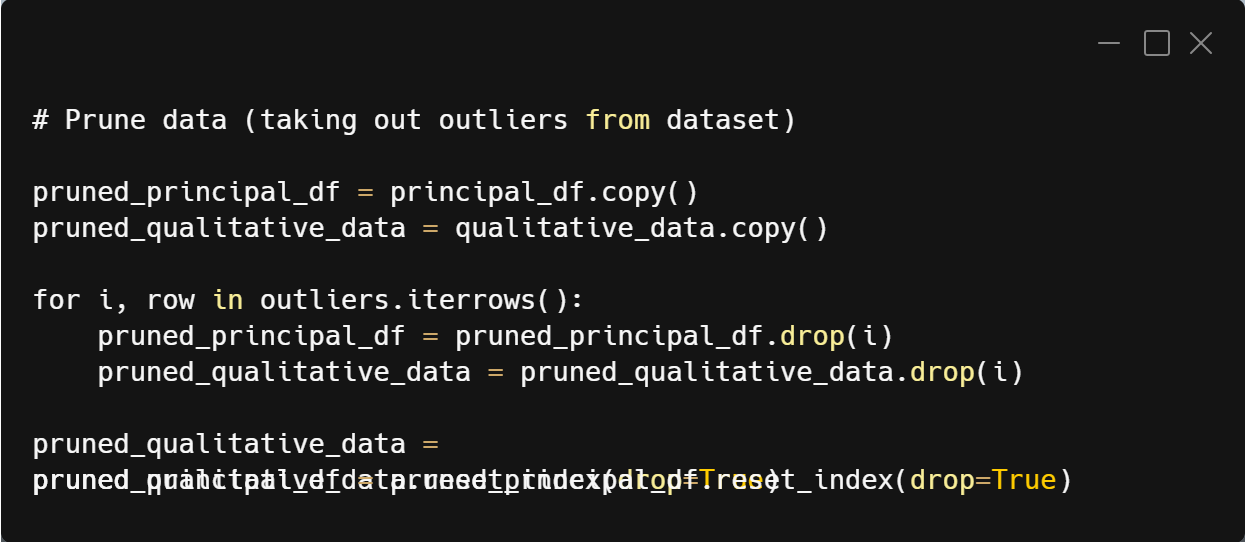
\includegraphics[width=\textwidth]{code4}
	\centering
	\caption{Code for pruning data}
\end{figure}
\vspace{-1em}
\begin{figure}[H]
	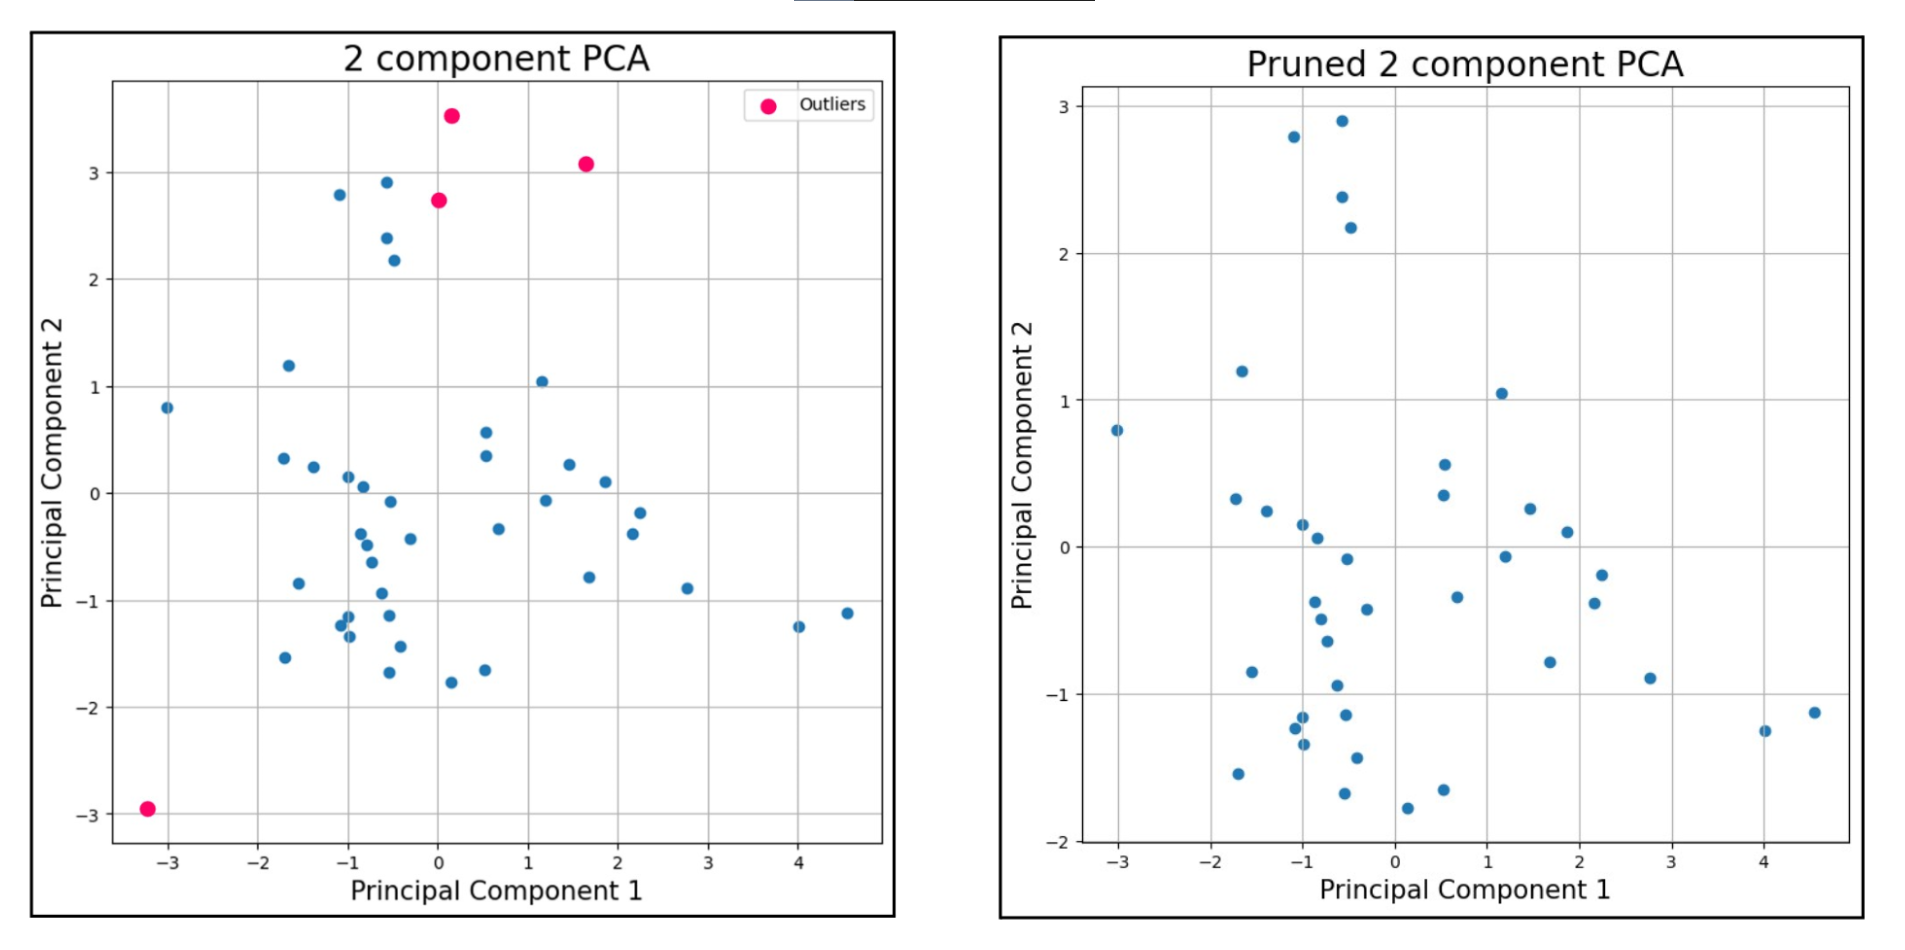
\includegraphics[scale=0.4]{6}
	\centering
	\caption{Resulting before \& after PCA plots}
\end{figure}

\subsection{Step 6: Visually analyze book scatterplot to estimate book distribution and groups}
Overall, after pruning the data, it is remarke that the points tend to cluster around certain areas. The final aim of the model is to classify books into ones that are “likely to be enjoyed” and “unlikely to be enjoyed” by me based on the factors I personally found influenced whether I would gravitate towards a book or not. Hence, it can be assumed that overall, the book points should fall into those two categories.

Visually examining the plot, however, it is noticed that there seems to be an additional point cluster towards the top. Referencing back to the book title labelled plot, manual estimates were made as to which category the books would fall into. The general areas are then highlighted, and the final image is presented here below:
\begin{figure}[H]
	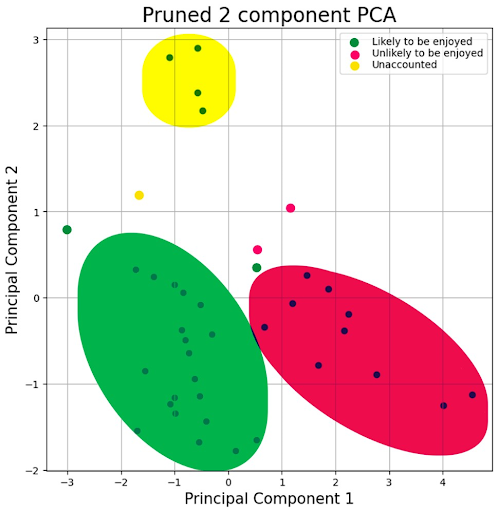
\includegraphics[scale=0.4]{7}
	\centering
	\caption{Highlighted estimated cluster regions for pruned PCA plot}
\end{figure}

\subsection{Step 7: Use KMeans clustering to generate cluster centre points}
This visual trend of points grouping, or clustering about specific points incites the use of a clustering algorithm such as KMeans to identify those coordinates. \parencite{2} This process is as follows:
\begin{enumerate}
    \itemsep -0.5em
    \item Firstly, the number of clusters (k) is chosen. Based on the visual analysis, k is determined to be $3$.
    \item Three random coordinates are then generated and plotted. All the points are assigned to one of these cluster centres based on which one is the closest.
    \item The cluster centre coordinates are re-computed and all the points re-assigned.
    \item This process is repeated again and again until the following criteria are met:
          \begin{enumerate}
            \itemsep -0.5em
            \item The new re-computed centre coordinates do not change.
            \item The points remain assigned to the same centre point.
          \end{enumerate} 
\end{enumerate}

These steps were applied to the dataset to yield the following centrepoints:

\begin{figure}[H]
	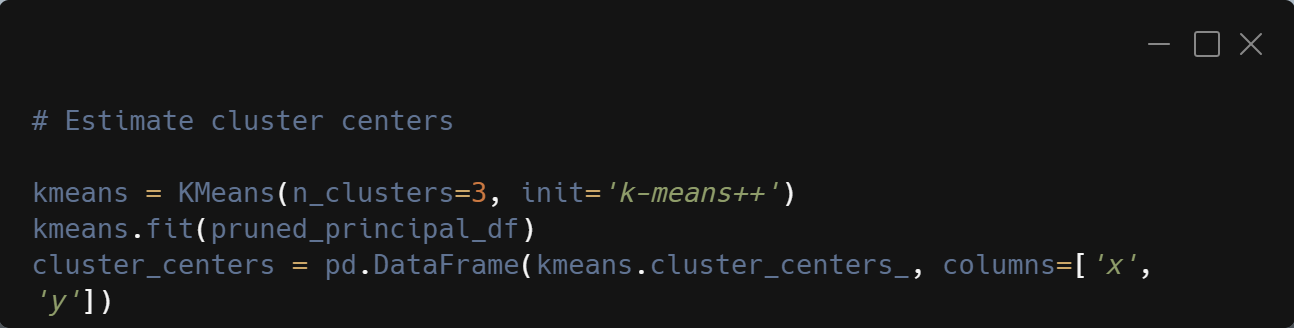
\includegraphics[width=\textwidth]{code5}
	\centering
	\caption{Code for KMeans}
\end{figure}
\vspace{-1em}
\begin{figure}[H]
	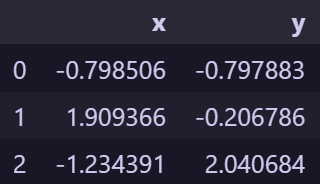
\includegraphics[scale=0.4]{8}
	\centering
	\caption{Calculated KMeans cluster centre coordinates}
\end{figure}

\subsection{Step 8: Plot cluster centre points}
The obtained coordinates of the cluster centre points from the previous step were then plotted and labelled with their appropriate category titles:

\begin{figure}[H]
	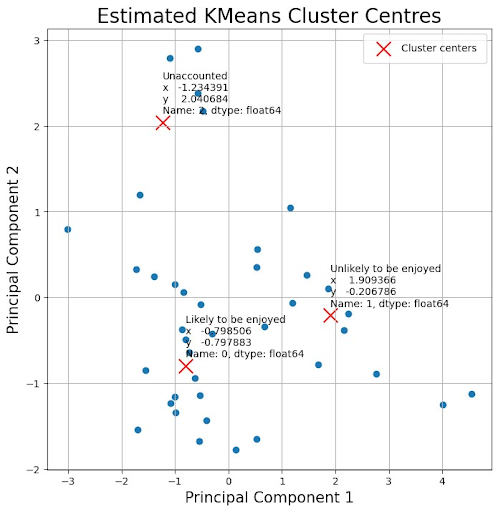
\includegraphics[scale=0.4]{9}
	\centering
	\caption{Plotted KMeans cluster centres}
\end{figure}

\subsection{Step 9: Construct a Voronoi diagram to form category cells}
As opposed to manually iterating through each point, determining its Euclidian distance to each centrepoint, and evaluating which category the point should be assigned to based on which is closest, a Voronoi diagram can be constructed. In the context of this IA, the centrepoints represent the Voronoi sites. Firstly the line intersections between the $3$ points are calculated and plotted. The programmed process and output graph is presented here below:

\begin{figure}[H]
	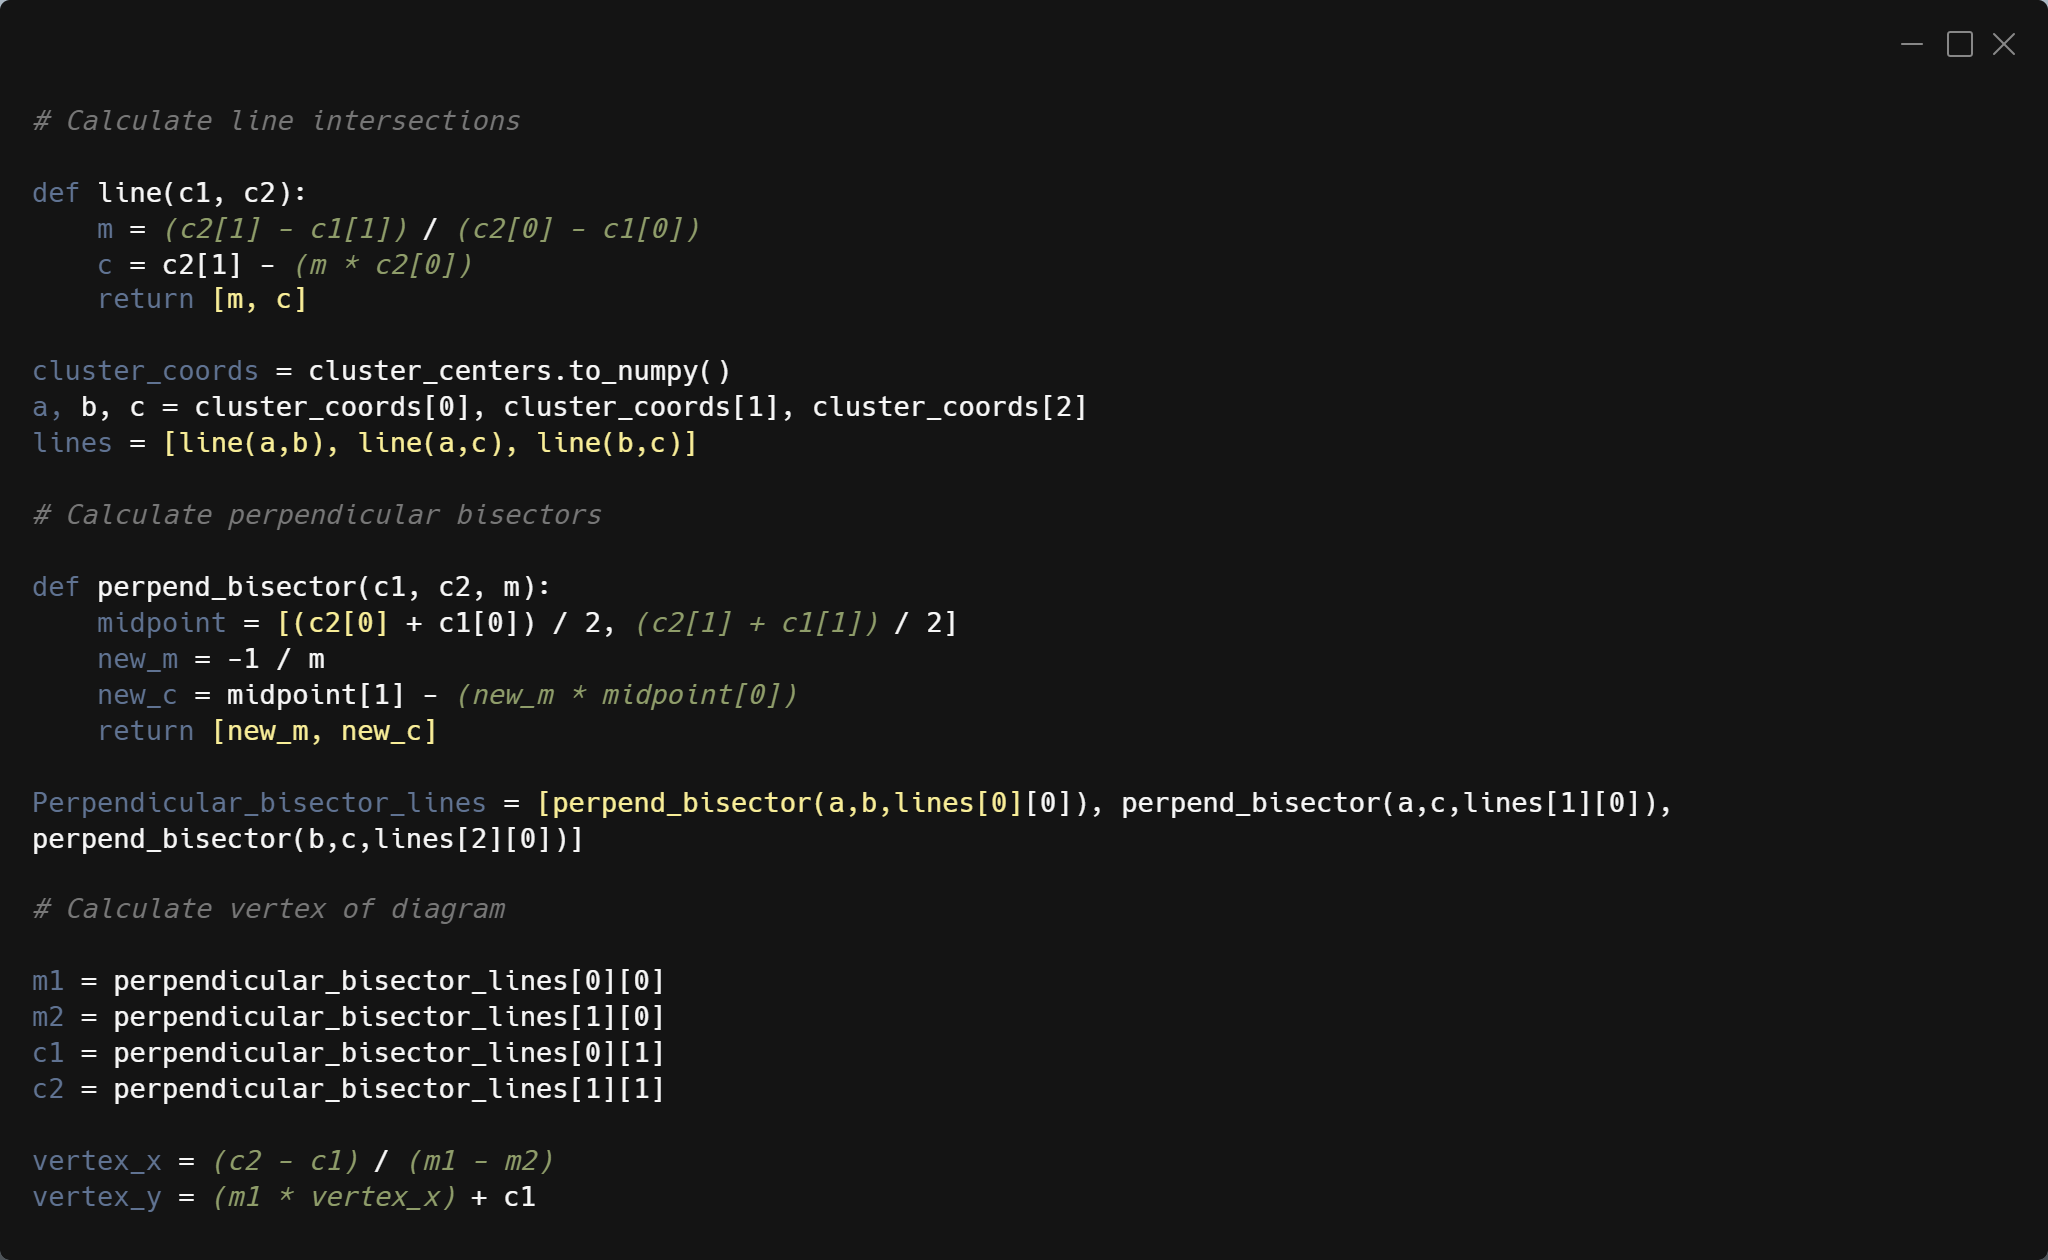
\includegraphics[width=\textwidth]{code6}
	\centering
	\caption{Code for constructing voronoi diagram}
\end{figure}
\vspace{-1.5em}
\begin{figure}[H]
	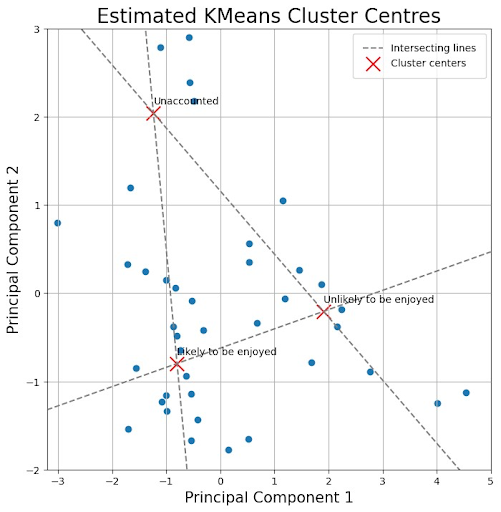
\includegraphics[scale=0.3]{10}
	\centering
	\caption{Plotted intersecting lines}
\end{figure}

After obtaining the line equations of the intersections centrepoint intersections, the perpendicular bisectors are calculated and plotted:

\begin{figure}[H]
	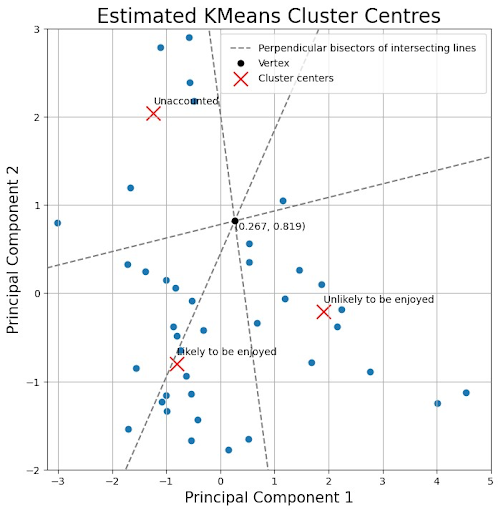
\includegraphics[scale=0.4]{11}
	\centering
	\caption{Plotted perpendicular bisectors of intersecting lines}
\end{figure}

Finally, the unused lines are removed, and the different cells colour-coded for ease of identification. The final model is presented here below:

\begin{figure}[H]
	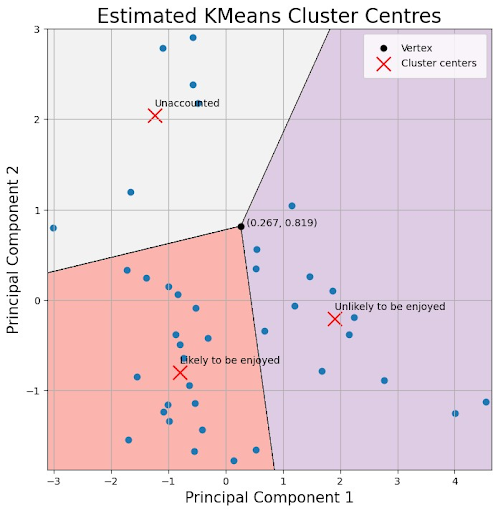
\includegraphics[scale=0.4]{12}
	\centering
	\caption{Final voronoi diagram}
\end{figure}

\pagebreak

\section{Reflections}
\begin{itemize}
    \item Despite the model being personalized to my preferences, the subjectivity of the choice of factors determining the “quality” of books may signify that the model cannot be used with other individuals and their own booklists, due to the high specificity of the model and its’ parameters.
    \item Following on from this, the model assumes that all the factors have equal “weighting” in the model (meaning that each variable is given the same degree of influence). A modification to improve this would be to introduce an option to vary the weighting of each variable.
    \item \parencite{3} To understand how much information was retained from performing PCA, the explained variance ratio is calculated. This represents the “usefulness” of the principal components. As a general rule, the percentage sum of the principal components should be around $0.8$. In total, the obtained variance ratio was found to be $0.52$, $0.29$ under the ideal value. Since this is not drastically low, this means that linear combinations of the variables can explain the factors’ variability only to an extent, so it is important to take this into consideration when determining the accuracy of the model.
    \item In the visual analysis of the scatter plot, an additional cluster of points was remarked and formed the “unaccounted” group. The presence of these points suggests that not all my preference factors were taken into account. Upon closer examination of the book titles, it was noticed that they all were non-fiction books. A modification that can be made to account for this is to add an additional factor: the“informative” mood percentage.
\end{itemize}

\section{Further Research}
\begin{itemize}
    \item The model’s accuracy can be tested with new points (recently finished books). The same process detailed in the procedure is applied to the points to yield principal components, which are then plotted onto the Voronoi diagram.
    \item Since the outcome of whether the book is enjoyed is known, the model’s accuracy can be determined by whether the points are plotted in the appropriate cells. This can be further extended by determining the Euclidian distance between the test data points and its’ corresponding group cluster centre point. As a general rule, the larger the distance between the two, the less accurate the model.
    \item As the model was simplified, it assumed equal weighting or “influence” of all the utilised factors on book preference. However, as was mentioned in the introduction, different factors hold varying importance for different individuals. Hence, it would prove interesting to explore how controlling the magnitude of the “influence” of certain factors on the model affects its’ predictive accuracy.
\end{itemize}

\section{Conclusion}
In conclusion, a model was constructed to address the aims detailed in the introduction. The steps which were followed were explained in terms of how they related to the aim, and how they would be carried out. Reflections were made on the weaknesses of the choices made, and modifications were suggested to improve on them. Finally, suggestions for further investigation and research are given that may improve the model.

\printbibliography[heading=bibintoc,title={References}]
\end{document}
